% mapgis2shp SoftwareX manuscript -- elsarticle / SoftwareX structure
\documentclass[preprint,12pt,numbers]{elsarticle}

\usepackage[T1]{fontenc}
\usepackage{booktabs}
\usepackage{tabularx}
\usepackage{amsmath}
\usepackage{amssymb}
\usepackage{url}
\usepackage{xcolor}
\usepackage{hyperref}
\usepackage{listings}
\usepackage{lineno}
\hypersetup{colorlinks=true,linkcolor=blue,citecolor=blue,urlcolor=blue}
\lstset{basicstyle=\ttfamily\small,breaklines=true,frame=single}
\journal{SoftwareX}

\begin{document}
\linenumbers
\begin{frontmatter}

\title{mapgis2shp: open-source interoperability and original-library rendering for legacy MapGIS 6.x/67 vector data}

\author[1]{Shijie Li\corref{cor1}}
\author[1]{Haiyang He\corref{cor2}}
\author[1]{Xu Sun}
\author[1]{Haoyang Qin}
\author[1]{Xiaoyu Liu}
\author[1]{Yilin Feng}
\author[1]{Zengyun Zuo}

\affiliation[1]{
  organization={Xi'an Mineral Resources Survey, China Geological Survey},
  city={Xi'an},
  country={China}
}
\cortext[cor1]{Co-corresponding author. Email: 1045105061@qq.com}
\cortext[cor2]{Co-corresponding author. Email: hehaiyangcugb@foxmail.com}

\begin{abstract}
Legacy MapGIS 6.x/67 files preserve geological mapping products, but their binary geometry, attributes and cartographic definitions are difficult to reuse. Geometry-only conversion also loses symbols, line styles, fill patterns and colours stored in separate libraries. Here we present \textbf{mapgis2shp} (import name \texttt{pymapgis}), an Apache-2.0 toolkit combining bidirectional vector interoperability, five-library parsing and original-library rendering. An external-fixture example pairs twelve user-supplied JWD layers with five matching SLIB files and produces PNG, PDF and SVG maps with machine-readable reports. It draws 5{,}732 original features from 7{,}094 inputs, excludes 1{,}362 fragmented annotations and reports zero unresolved colours, fills, fallbacks or symbols. A coordinate test retains all 782 source vertices in 37 real features, with maximum deviation $\leq 10^{-9}$ in source units. With external fixtures, local regression comprises 423 passing tests and one environment-dependent skip; continuous integration covers four platforms and release checks. Version 2.7.1 is available through PyPI, GitHub and Zenodo. Historical Reader comparisons cover 36 survey layers and a 400~MB polygon dataset. The result is an auditable route from closed MapGIS binaries to open vector processing and original-library rendering, without treating internal regression as vendor-identical visual acceptance.
\end{abstract}

\begin{keyword}
MapGIS \sep vector interoperability \sep graphic-library parsing \sep original-library rendering \sep GeoPandas \sep geological survey \sep open source
\end{keyword}
\end{frontmatter}

\section{Motivation and significance}

\subsection{Legacy interoperability as a scientific-data problem}

MapGIS 6.x/67 binary vector files remain common in Chinese geological surveying, mineral-resource assessment and engineering geology~\cite{ma2012,han2012}. They encode not only coordinates and attributes but also references to cartographic libraries that control how a geological map is intended to appear. The closed nature of these formats impedes reproducible analysis, cross-platform quality control and long-term preservation. Official exports can recover parts of the data, yet they may discard coordinate-reference metadata, numeric precision, text padding and native display definitions.

This work addresses two linked requirements. First, researchers need reliable vector interoperability: reading, converting and writing point, line and polygon files without silently changing their geometry or attributes. Second, they need to inspect and reconstruct the original cartography, not merely an approximate map generated from replacement colours and line styles. The second requirement makes the originating graphic libraries part of the research data itself.

\subsection{From a reader to an auditable open mapping stack}

Earlier versions of mapgis2shp concentrated on the reader path and native-export comparison. Version 2.7.1 extends that core with native writing, five-library parsing, original-library rendering and documented regression fixtures. The intended result is not a pixel-identical replacement for the MapGIS application. It is an open and inspectable implementation whose assumptions can be tested: binary offsets are explicit, colour channels are selected deliberately, unresolved structures remain non-results, and rendered coordinates can be compared with the source vertices.

Figure~\ref{fig:architecture} summarises this transition from an opaque source package to vector conversion, library interpretation and evidence-based validation.

\begin{figure}[htbp]
\centering
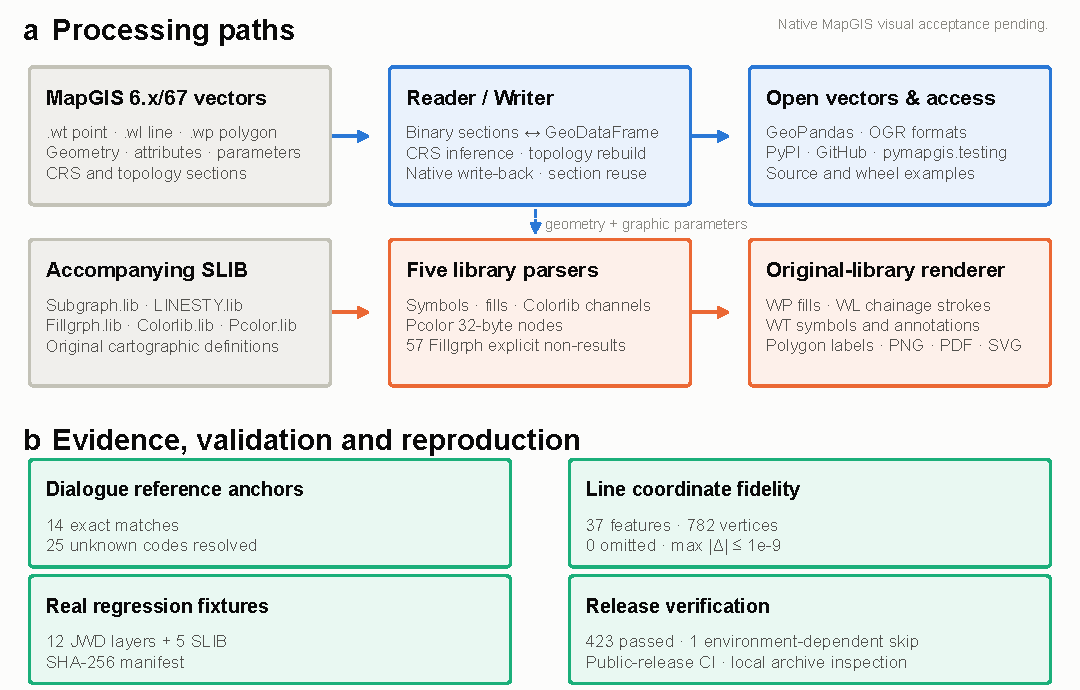
\includegraphics[width=\textwidth]{softwarex_architecture}
\caption{Architecture and verification paths of mapgis2shp 2.7.1. \textbf{(a)} Reader/Writer exchanges MapGIS vectors with GeoDataFrames, OGR formats and native write-back. Original-library rendering combines those data with Subgraph, LINESTY, Fillgrph, Colorlib and Pcolor definitions. \textbf{(b)} Colour anchors, coordinate checks, external JWD/SLIB and release inspection provide separate evidence layers; internal regression is not native MapGIS visual acceptance.}
\label{fig:architecture}
\end{figure}

\subsection{Relation to existing tools}
The official GDAL/OGR vector-driver index does not list a driver for the legacy MapGIS binary formats, leaving the usual open-source vector-I/O path unavailable for these files~\cite{gdalwebsite,warmerdam2008}. Earlier open-source efforts include the first author's predecessor reader \texttt{pymapgis}~\cite{pymapgis2022}, the record-level MapGIS2ArcGIS implementation~\cite{mathsionyang2019}, the independent ConvertMapGIS derivative~\cite{convertmapgis2025} and OGC.net~\cite{ogcnet2021}. The present contribution is therefore not a claim of priority for byte-level parsing alone. It combines a maintained bidirectional vector interface, five original-library parsers, coordinate-faithful rendering and real-data regression in one installable package. This evidence-guided approach follows a broader pattern of open scientific-format interoperability tools such as \texttt{sas7bdat} and \texttt{python-ags4}~\cite{shotwell2011,senanayake2022}.

\section{Software description}

\subsection{Architecture and public interfaces}

The package exposes four groups of functionality:
\begin{enumerate}
  \item \textbf{Vector interoperability.} \texttt{Reader}, \texttt{Writer} and \texttt{write()} exchange \texttt{.wt}, \texttt{.wl} and \texttt{.wp} files through GeoPandas GeoDataFrames and OGR-supported formats.
  \item \textbf{Graphic-library parsing.} \texttt{SubgraphLib}, \texttt{LinestyLib}, \texttt{FillgrphLib}, \texttt{ColorLib} and \texttt{PcolorLib} decode the five original library files.
  \item \textbf{Original-library rendering.} \texttt{GraphicLibraries}, \texttt{GraphicRenderer}, \texttt{GraphicRenderResult} and \texttt{render\_graphic\_map()} render WP, WL and WT layers using those parsed definitions.
  \item \textbf{Reproducibility.} \texttt{pymapgis.testing} locates bundled synthetic and Writer fixtures and resolves external JWD/SLIB directories through explicit environment paths. The command-line interface converts vectors and inspects all five library types.
\end{enumerate}

Geological interpretation, contact or fault classification, GeoSciML conversion~\cite{sen2005} and thematic recolouring presented as native MapGIS output are deliberately outside the package's format-level responsibility. Attribute-derived labels are supported as a display operation, not as a geological semantic transformation.

\subsection{Vector Reader and Writer}

The Reader consumes 16 physical section-index entries and reconstructs attributes, geometries and optional graphic parameters in an aligned GeoPandas GeoDataFrame~\cite{geopandas}. Coordinate-reference inference uses pyproj~\cite{pyproj} and covers longitude/latitude, Transverse Mercator, Albers and Lambert conventions, with non-finite or invalid projection parameters falling back to an empty CRS rather than plausible-looking but corrupted coordinates. Polygon reconstruction uses Shapely~\cite{shapely} to assemble shells and holes from arc--node topology while filtering orphan topology identifiers consistently across attributes, geometry and graphic parameters.

The Writer supports native point, line and polygon output. Unchanged geometry and metadata from a Reader can reuse original sections verbatim. Freshly authored polygons use independently closed rings and native 24-bit ring-index pointers; raw-ring preservation is the default, with \texttt{shapely.make\_valid} available only on request. Because MapGIS 6.x cannot encode the UTM scale factor, UTM input is reprojected to Gauss--Kruger with $k=1$ and a runtime warning; round-trip checks transform back to the original CRS. Reader--Writer--Reader checks are treated as internal regression, not as proof of native MapGIS acceptance.

\subsection{Graphic-library parsing}

Table~\ref{tab:libraries} lists the library roles and current decoding coverage. Unsupported or unconventional records remain explicit non-results instead of being replaced by guessed geometry.

\begin{table}[htbp]
\centering
\caption{Graphic-library roles and current structural coverage.}
\label{tab:libraries}
\small
\begin{tabularx}{\textwidth}{@{}llX@{}}
\toprule
Library & Rendering role & Verified structural result \\
\midrule
Subgraph.lib & Point symbols and element groups & 7{,}360 structural records enumerated \\
LINESTY.lib & Subline variants, rhythms and pens & 859 non-empty styles; 984 sublines \\
Fillgrph.lib & Polygon fill patterns & 1{,}280/1{,}337 records; 57 explicit non-results \\
Colorlib.lib & Pattern, line, auxiliary and point colours & 871 entries with explicit KCMY/YMCK models \\
Pcolor.lib & WP fills and extended colours & 4{,}098 32-byte colour nodes \\
\bottomrule
\end{tabularx}
\end{table}

\subsection{Original-library rendering}

The Matplotlib-based renderer~\cite{matplotlib} preserves polygon holes, instantiates fill-pattern tiles, stamps line-style elements along original vector geometry, instantiates Subgraph symbols and renders text annotations. WP fills use Pcolor by default when available; other colour roles continue to use Colorlib. Main and independent auxiliary line records are decoded separately, while in-range auxiliary values select main-record variants rather than producing an extra line.

Complete geological-unit labels can be generated from polygon attributes at \texttt{representative\_point()}, using MapGIS control codes and Mathtext for subscripts and superscripts. This presentation choice avoids duplicating fragmented WT \texttt{CHFCEC=unit-code} annotations. Other annotation categories, native text advances, negative spacing and native font-number mappings remain supported.

\section{Illustrative examples}

\subsection{Installation and basic use}

The package is available on PyPI; Matplotlib is required only for the rendering extra:
\begin{lstlisting}
python -m pip install "mapgis2shp[render]"
\end{lstlisting}

Obtain the original vectors and libraries through their official channel and set \texttt{PYMAPGIS\_JWD} and \texttt{PYMAPGIS\_SLIB} before running the example. In the current wheel, replace \texttt{examples} with \texttt{pymapgis.testing.examples} in the first import below; the source archive retains the shown \texttt{examples/} layout. The published V2.7.1 wheel is checked separately through \texttt{validate\_published\_quickstart.py}, which reads the fixtures directly with \texttt{Reader}.
\begin{lstlisting}[language=Python]
import examples.render_bundled_jwd as jwd
from pymapgis import GraphicLibraries, GraphicRenderer
from pymapgis.testing import jwd_path, slib_path

libraries = GraphicLibraries.from_directory(slib_path())
renderer = GraphicRenderer(
    libraries,
    scale=250000,
    native_text_layout=True,
    polygon_labels=True,
    polygon_label_fontsize=5.0,
    polygon_label_scale=0.7,
    text_font_family=["Microsoft YaHei", "SimSun", "DejaVu Sans"],
    font_zh_map={1: "SimSun", 4: "SimHei"},
    font_en_map={0: "DejaVu Sans"},
)
layers = jwd.regression_layers(jwd_path())
result = renderer.render(layers, "map.png", figsize=(12, 7.5), dpi=600)
print(result.reports)
\end{lstlisting}

Here \texttt{jwd\_path()} and \texttt{slib\_path()} resolve external user-supplied Kurgan-sheet vectors (JWD) and graphic-library directories (SLIB) without hard-coded absolute paths. Reports distinguish 5{,}732 drawn original features from 1{,}362 excluded fragmented WT unit-code annotations, totalling 7{,}094 inputs. Users should check \texttt{unknown\_colors}, \texttt{symbols\_unresolved} and \texttt{unknown\_fonts}, together with \texttt{unknown\_fill}, \texttt{fallback}, \texttt{empty\_pattern} and \texttt{cycle\_limit} and their emitted \texttt{aux\_} counterparts, for empty or zero results. Chinese annotations require a CJK-capable font.

The executable \texttt{examples/render\_bundled\_jwd.py} additionally writes PDF and SVG maps and \texttt{jwd\_render\_reports.json}. Figure~\ref{fig:rendered-example} shows the resulting map.

% When a new release is produced, keep the fixture inventory and example
% synchronized with the release archive and this compatibility path.

\begin{figure}[htbp]
\centering
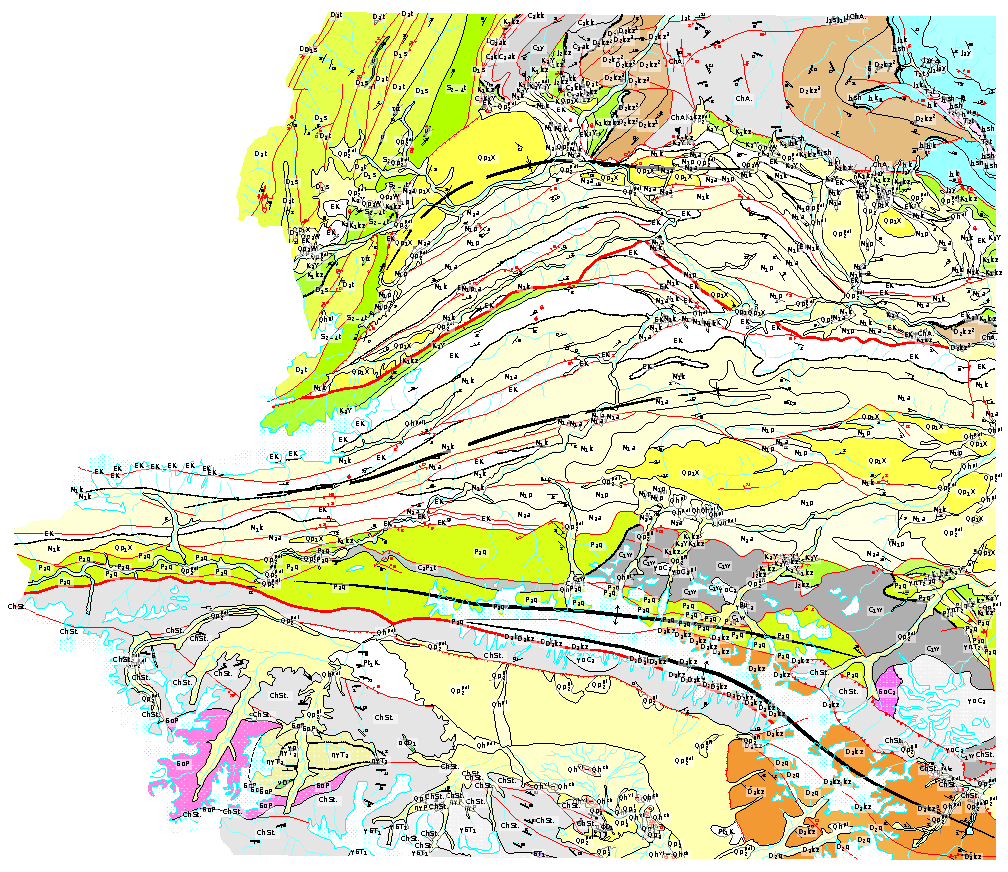
\includegraphics[width=\textwidth]{jwd_map}
\caption{Original-library output from user-supplied JWD/SLIB regression data. The public example drew 5{,}732 features and generated 713 polygon labels from 7{,}094 inputs, excluding 1{,}362 fragmented annotations, with zero unresolved colours, fills, fallbacks, symbols or fonts. No scale bar, north arrow, graticule or legend is drawn. The tightly cropped vector PDF/SVG supports enlargement; dense native annotations and label--line-work overlaps remain. This is internal regression output, not native MapGIS visual acceptance.}
\label{fig:rendered-example}
\end{figure}

\section{Implementation and evidence-based parsing}

\subsection{Pcolor node recovery and colour-role separation}

Colour decoding follows physical 32-byte nodes rather than inferred slots. Colour number $N$ maps to node $N+3$, with K/C/M/Y channels at node offset 28. Only out-of-range numbers return no colour, because all-zero KCMY can represent valid white. This model reproduces 14 reference anchors recorded from the native colour dialogue and resolves all 25 previously unresolved colour codes and their 418 fallback occurrences without unit-specific overrides. WP fills use Pcolor by default, while other colour roles use Colorlib with an explicit KCMY or YMCK model rather than automatic channel switching.

\subsection{LINESTY variants and auxiliary semantics}

Line-style decoding uses element templates and f32 payload offsets rather than line numbers alone. An in-range auxiliary style number selects a main-record subline variant, whereas an out-of-range value identifies an independent auxiliary record, with a documented exception for the style-2 equivalent-dash family. This prevents 16\textbar1 from acquiring an unintended baseline and selects subline four for 65\textbar4 with six fill units and a 30.4~mm period. Unsupported variants remain unresolved rather than being replaced by guessed geometry.

\subsection{Coordinate-faithful line rendering}

Zero-offset strokes are clipped by source chainage, retaining every original vertex in the clipped interval. Constant-offset strokes use complete offset curves, with rhythm phase measured on the original line rather than on the longer or shorter offset curve. A dedicated path preserves the continuous baseline and actual library intervals for the 48\textbar0 parallel-unconformity style, while zero-longitudinal-length ticks use a half-open interval $[0,\mathrm{total})$. A direct source-coordinate test checks 37 real 38\textbar2 features, where 38\textbar2 denotes linetype 38 with auxiliary style number 2.

\subsection{Validation fixtures and reproducibility}

The distribution includes synthetic and Writer interoperability fixtures, attribution files and SHA-256 manifests, but not the original JWD, SLIB or native SHP data. Users supply those external datasets through \texttt{PYMAPGIS\_JWD}, \texttt{PYMAPGIS\_SLIB} and \texttt{PYMAPGIS\_READER\_NATIVE}. Missing external data produces an explicit optional-integration skip with acquisition guidance; missing required Writer fixtures or any checksum mismatch fails the test. Archive inspection rejects the original data files.

The twelve-layer fixture is a subset of the public, non-classified \emph{Spatial database of serial suite-tectonic map-sheets of mainland China (1:250,000)} (V1), produced by the Development and Research Center of China Geological Survey and distributed by the National Geological Archives of China~\cite{dataset2018,datasetpaper2018}. Its accompanying SLIB supplies the original symbol, line-style, fill-pattern and colour definitions; no unrelated MapGIS installation library is substituted. Current regression and the rendered example use only the original open-edition JWD and SLIB, not coordinate-warped or virtual-geological-unit derivatives.

\section{Validation and reproducibility}

\subsection{Current regression evidence}

Table~\ref{tab:validation} separates current structural and rendering checks from historical Reader evidence. The example runs from a source checkout and the current wheel with external fixtures, and Figure~\ref{fig:rendered-example} is generated by that public example. The workflow runs it when external fixture directories are configured and otherwise prints an explicit optional-data skip.

\begin{table}[htbp]
\centering
\caption{Current validation evidence and its meaning.}
\label{tab:validation}
\small
\begin{tabular}{p{0.37\textwidth}p{0.53\textwidth}}
\toprule
Evidence & Result and interpretation \\
\midrule
Full package regression & With external fixtures, 423 passed and 1 environment-dependent skip; without them, 394 passed and 13 optional skips locally with Python 3.12.7, GeoPandas 1.1.3 and Matplotlib 3.9.2 \\
Continuous integration & Run \href{https://github.com/leecugb/mapgis2shp/actions/runs/42613725710}{42613725710} passed on Python 3.9 on Ubuntu and Python 3.13 on Ubuntu, Windows and macOS at commit \texttt{95ecc53}; archive building, content inspection and Twine checks also passed. Real JWD rendering was optional-skipped on runners without external data \\
Real twelve-layer rendering & 7{,}094 inputs; 5{,}732 drawn and 1{,}362 excluded; no unresolved colours, unknown fills or solid fallbacks \\
Native dialogue reference anchors & All 14 reference anchors recorded from the native colour dialogue match; all 25 previous unknown colour codes resolved \\
38\textbar2 coordinate fidelity & All 37 features and all 782 source vertices retained; maximum vertex deviation $\leq 10^{-9}$ in source coordinate units (geographic degrees for this dataset) \\
Execution states & Published PyPI V2.7.1 Quickstart passed; with external fixtures, 79 targeted rendering, Reader and Writer tests passed in source and current wheel states \\
Archive verification & 291 wheel entries and 329 source-archive entries pass content inspection in the external-fixture revision build \\
\bottomrule
\end{tabular}
\end{table}

Current tests cover topology, auxiliary rhythms, symbols, text layout, fonts, Mathtext, DPI conversion and unresolved variants. A census test asserts the totals in Table~\ref{tab:libraries}. Forty-three native SHP cases verify Writer attributes, polygon topology, default styles, UTM round-trips, null/degenerate inputs and 24-bit ring-index bounds. Native anomalies are counterexamples, not behaviour to inherit. Five additional export groups test Reader coverage, attribute fidelity and validity, including recovery of a polygon absent from SHP. Manifest and non-empty-inventory checks fail for missing, empty or altered fixtures. The 36-file Reader--Writer--Reader smoke suite also passed with zero area relative difference. It used the 12 original JWD layers and 24 additional layers from the same open sheet. All 36 are external and none is redistributed in the current package; they must be obtained separately. These checks establish internal consistency rather than vendor-identical rendering.

\subsection{Historical native-export validation}

Earlier Reader-only experiments covered 36 real survey layers containing 16{,}874 features. Feature counts and attribute schemas matched, aligned geometries met the type-specific coincidence criteria, and mean layer-level attribute equivalence was 99.9995\%. Two mismatches among 95{,}006 compared cells were consistent with coarse native-export rounding. A separate 400~MB dataset with 78{,}873 features achieved 99.73\% coverage intersection-over-union and zero invalid geometries, compared with three in the post-processed reference export. Reconstruction overlaps increased summed polygon areas by 1.66\%, whereas union-level coverage differed by 0.27\%. These remain historical Reader results, not renderer validation. Scripts and reports are preserved under \texttt{paper/validation/} at commit \texttt{d0d464d0}, with a permanent entry point at \url{https://github.com/leecugb/mapgis2shp/tree/d0d464d05166ab97978a01ce8cc5cc8480f05500}.

\section{Impact}

The package supports several research workflows:
\begin{itemize}
  \item migrating legacy vectors to open formats and writing native files for subsequent MapGIS acceptance checks;
  \item reconstructing original cartography and comparing colours, line styles, patterns and labels with reference evidence;
  \item auditing coordinate fidelity and conversion-induced information loss;
  \item teaching binary-format interoperability and evidence-guided reverse engineering through reproducible examples.
\end{itemize}

Externally supplied vectors and SLIB make the complete parser and rendering path reproducible after official acquisition. For other datasets, users must supply libraries from the originating installation. The original SLIB remains a regression reference, not a redistributed universal replacement for library-local definitions.

\section{Limitations and verification boundaries}

Structural coverage does not imply pixel-identical MapGIS output. A full native visual comparison of all 859 non-empty line styles has not yet been performed. Fifty-seven unconventional Fillgrph records remain explicit non-results. Transparent-output and non-zero auxiliary-flag paths are not exercised by the present sheet, and other MapGIS installations may contain different library versions or colour models.

The historical 36-layer and 400~MB native-export results must not be extrapolated to every producer, object type or export configuration. Polygon reconstruction can still require repair for topological gaps. Native MapGIS opening, editing and save/reopen acceptance of newly written files remains a separate verification step. Versioned capture provenance for the 14 native-dialogue colour anchors also remains a submission requirement; current tests verify the recorded RGB values, not the completeness of their capture history. Text script metrics, font substitution and \texttt{representative\_point()} labels are display-level choices rather than proof of identical native layout. The dense JWD sheet retains native annotation placement, including label--line-work overlaps, so its automated collision audit remains a diagnostic rather than a passed production-layout check. Some native annotation sizes fall below common journal figure guidelines, so the vector PDF/SVG should be used for enlargement rather than raster downsampling.

The original Beijing-54 coordinate system and 1956 elevation datum used by the dataset also require attention in downstream research. Conversion to CGCS2000 and the 1985 national elevation datum may be necessary, and the source material is limited to data available through 2013 with only basic national coverage.

\section{Conclusions}

Mapgis2shp connects legacy MapGIS binaries to an inspectable open-source workflow for vector conversion, original-library parsing and cartographic rendering. The original JWD/SLIB example, native conversion counterexamples and explicit non-results make the implementation and its boundaries reproducible rather than implicit. Remaining work includes native MapGIS visual acceptance, fuller library-version coverage and item-level redistribution confirmation; these tasks are kept separate from the evidence already established.

\section{Availability and requirements}

\begin{table}[htbp]
\centering
\caption{Code metadata for the software described in this article.}
\label{tab:code-metadata}
\footnotesize
\begin{tabular}{p{0.07\textwidth}p{0.25\textwidth}p{0.60\textwidth}}
\toprule
Item & Metadata field & Value \\
\midrule
C1 & Current code version & 2.7.1 public release commit \texttt{823a5daf059c91d2a5ec90a685219d108519ae22}; manuscript validation uses the post-release integration state in C2 \\
C2 & Permanent link to code/repository used for this version & \url{https://github.com/leecugb/mapgis2shp/releases/tag/V2.7.1}; \url{https://doi.org/10.5281/zenodo.24036158}; regression example and hash manifests at \url{https://github.com/leecugb/mapgis2shp/tree/f9ca6a6675b899d282f1f5c407056c0e83f634c2} \\
C3 & Permanent link to reproducible capsule & The example, hash manifests and generated reports accompanying this manuscript serve as the capsule; original JWD/SLIB data are obtained separately through the official channel. \texttt{examples/render\_bundled\_jwd.py} and \texttt{mapgis2shp\_submission/validate\_published\_quickstart.py} are available from the integration commit in C2; generated maps and JSON reports also accompany the manuscript. \\
C4 & Legal code license & Apache-2.0 for the software; source vectors and SLIB retain their original terms \\
C5 & Code versioning system & Git and GitHub \\
C6 & Languages, tools and services & Python; GeoPandas, Shapely, NumPy, pandas, pyproj, pyogrio and Matplotlib; PyPI and GitHub Actions \\
C7 & Environments and dependencies & Python $\geq$ 3.9; geopandas $\geq$ 0.12, numpy $\geq$ 1.21, pandas $\geq$ 1.3, pyogrio $\geq$ 0.8, pyproj $\geq$ 3.2 and shapely $\geq$ 2.0; matplotlib $\geq$ 3.5 for rendering; Windows, Linux and macOS \\
C8 & Developer documentation & \url{https://github.com/leecugb/mapgis2shp#readme} and the repository \texttt{docs/} directory \\
C9 & Support email & \texttt{1045105061@qq.com}; \texttt{hehaiyangcugb@foxmail.com} \\
\bottomrule
\end{tabular}
\end{table}

% When a new release is produced, advance C1-C3 together with the
% corresponding regression artifacts and compatibility validation.

\section{Data availability and provenance}

The real regression uses external original layers from the Kurgan sheet (J43C001002) of the \emph{Spatial database of serial suite-tectonic map-sheets of mainland China (1:250,000)} (V1), produced by the Development and Research Center of China Geological Survey and distributed by the National Geological Archives of China. The dataset and companion article are identified by DOI \texttt{10.23650/data.A.2018.NGA131703.K1.1.1.V1} and \texttt{10.12029/gc2018Z101}~\cite{dataset2018,datasetpaper2018}. Users obtain the 12 vectors and five matching SLIB libraries through the official service at \url{http://dcc.cgs.gov.cn} and set \texttt{PYMAPGIS\_JWD} and \texttt{PYMAPGIS\_SLIB}; native SHP checks use \texttt{PYMAPGIS\_READER\_NATIVE}. Current source trees, wheels and source archives do not include those original data. Hash manifests, the example, generated maps and JSON reports accompany this manuscript without coordinate-warped or virtual-unit variants.

Public access, non-classified status and test-only use do not grant redistribution. The publishing-system policy requires a written agreement for dissemination, and its order-service notice prohibits third-party provision and internet redistribution~\cite{ngacsharing2017,ngacorder,ngacpolicy}. Earlier public V2.7.1 artifacts and historical commits contained covered files; removing them from the current tree does not erase those copies. Their remediation is documented separately in \texttt{ngac\_distribution\_remediation\_plan.md}. The software licence does not relicense the source data. The full 729-sheet database and historical 400~MB dataset are not redistributed by this work.


\section{Author declarations}

\subsection*{CRediT author statement}

S.L. conceived and designed the study, developed the software, carried out the validation and wrote the main manuscript text; S.L. also prepared the original figures. H.H. contributed to the validation and reviewed the manuscript. X.S., H.Q., X.L., Y.F. and Z.Z. contributed to data investigation and reviewed the manuscript. All authors reviewed and approved the previous manuscript version.


\subsection*{Declaration of competing interests}

The authors declare no competing interests.

\subsection*{Funding}

This work was supported by the Deep Earth Probe and Mineral Resources Exploration - National Science and Technology Major Project (Program No.2025ZD10069).

\begin{thebibliography}{99}

\bibitem{dataset2018}
Zuo Q, Ye T, Feng Y, Ge Z, Wang Y (2018) Spatial database of serial suite-tectonic map-sheets of mainland China (1:250,000) (V1). Development and Research Center of China Geological Survey [producer], 2006. National Geological Archives of China [distributor], 2018-09-10. \url{https://doi.org/10.23650/data.A.2018.NGA131703.K1.1.1.V1}

\bibitem{datasetpaper2018}
Zuo Q, Ye T, Feng Y, Ge Z, Wang Y (2018) Spatial database of serial suite-tectonic map-sheets of mainland China (1:250,000). Geology in China 45(S1):1--26. \url{https://doi.org/10.12029/gc2018Z101}

\bibitem{ngacpolicy}
National Geological Archives of China (2025) Measures for geological data services. \url{https://www.ngac.cn/125cms/c/qggnew/fwgl_t.htm?id=0&isnull=N}. Accessed 7 November 2026.

\bibitem{ngacsharing2017}
Li C, Wu X, Qi F, et al. (2017) Exploration and research on the global geological data publishing model. Geology in China 44(S1):1--7. \url{https://doi.org/10.12029/gc2017Z101}

\bibitem{ngacorder}
National Geological Archives of China. Nationwide online order service instructions for geological data (trial). \url{https://www.ngac.cn/125cms/c/qggnew/dzzlwlddfwxz.htm}. Accessed 9 November 2026.

\bibitem{pymapgis2022}
Li S (2022) pymapgis: a Python library for reading MapGIS 6.x/67 vector files. \url{https://github.com/leecugb/pymapgis}. Accessed 22 July 2026.

\bibitem{gdalwebsite}
GDAL/OGR contributors (2026) Vector drivers list. \url{https://gdal.org/drivers/vector/index.html}. Accessed 22 July 2026.

\bibitem{warmerdam2008}
Warmerdam F (2008) The Geospatial Data Abstraction Library. In: Hall GB, Leahy MG (eds) Open Source Approaches in Spatial Data Handling. Advances in Geographic Information Science. Springer, Berlin, Heidelberg, pp 87--104. \url{https://doi.org/10.1007/978-3-540-74831-1_5}

\bibitem{mathsionyang2019}
MathsionYang (2019) MapGIS2ArcGIS. \url{https://github.com/MathsionYang/MapGIS2ArcGIS}. Accessed 22 July 2026.

\bibitem{convertmapgis2025}
BenChao1998 (2025) ConvertMapGIS. \url{https://github.com/BenChao1998/ConvertMapGIS}. Accessed 22 July 2026.

\bibitem{ogcnet2021}
Wong W (2021) OGC.net. \url{https://github.com/WenboWong/OGC.net}. Accessed 22 July 2026.

\bibitem{geopandas}
GeoPandas contributors (2026) GeoPandas: geographic extensions to pandas. \url{https://geopandas.org/}. Accessed 7 November 2026.

\bibitem{shapely}
Gillies S (2026) Shapely: manipulation and analysis of geometric objects. \url{https://shapely.readthedocs.io/}. Accessed 7 November 2026.

\bibitem{pyproj}
Pyproj contributors (2026) pyproj: Python interface to PROJ. \url{https://pyproj4.github.io/pyproj/}. Accessed 7 November 2026.

\bibitem{matplotlib}
Hunter JD (2007) Matplotlib: a 2D graphics environment. Computing in Science \& Engineering 9(3):90--95. \url{https://doi.org/10.1109/MCSE.2007.55}

\bibitem{sen2005}
Sen M, Duffy T (2005) GeoSciML: development of a generic GeoScience Markup Language. Computers \& Geosciences 31(9):1095--1103. \url{https://doi.org/10.1016/j.cageo.2004.12.003}

\bibitem{shotwell2011}
Shotwell M (2011) sas7bdat: sas7bdat reverse engineering documentation. CRAN (The R Foundation). \url{https://doi.org/10.32614/cran.package.sas7bdat}

\bibitem{senanayake2022}
Senanayake AI, Chandler RJ, Daly T, Lewis E (2022) python-ags4: a Python library to read, write, and validate AGS4 geodata files. Journal of Open Source Software 7(79):4569. \url{https://doi.org/10.21105/joss.04569}

\bibitem{ma2012}
Ma Y, Wang J, Xie S (2012) Analytical application of MapGIS for quality control in geological map spatial database constructing. Geo-information Science 13(6):758--762. \url{https://doi.org/10.3724/sp.j.1047.2011.00758}

\bibitem{han2012}
Han K, Pang J, Lu Y, Ding D, Fan B, Ju Y, Wang Z (2012) Research on sharing of geological map spatial data network under the ``OneGeology'' project: taking China 1:1M geological map data in MapGIS format as an example. Geo-information Science 13(6):742--749. \url{https://doi.org/10.3724/sp.j.1047.2011.00742}

\end{thebibliography}

\end{document}
